\chapter{Incertitude, théorème d’Ehrenfest et limite classique}

\section{Le problème en suspens de l’Hamiltonien linéaire}

Le modèle
\begin{equation}
H=cP
\label{eq:l10-linear-hamiltonian}
\end{equation}
était utile parce que ses paquets d’ondes se translatent sans changer de forme. Il comporte aussi une sérieuse mise en garde. L’impulsion peut être positive ou négative : la même formule attribue donc une énergie positive à une onde plane et une énergie négative à l’autre :
\begin{equation}
\psi_p(x)=e^{ipx/\hbar},
\qquad
E(p)=cp.
\end{equation}
Si un nombre arbitraire de particules physiques pouvait occuper des états d’énergie négative, le vide ne serait pas l’état d’énergie minimale. Il pourrait produire des quanta d’énergie positive tout en déposant une énergie négative compensatrice dans de nouvelles particules : l’énergie totale serait conservée, mais l’énergie du vide pourrait diminuer sans limite.

\begin{classroomqa}
\audiencequestion{Pourquoi une branche d’énergie négative est-elle plus qu’un choix étrange de l’origine des énergies ?}
\lecturerresponse{Ajouter la même constante à toutes les énergies est sans conséquence. Un spectre non borné est une autre affaire. Si l’on peut peupler des états d’énergie toujours plus basse tandis que des particules d’énergie positive emportent l’énergie compensatrice, il n’existe aucun état fondamental stable. La stabilité exige que l’énergie soit minorée par rapport au vide.}
\end{classroomqa}

\begin{figure}[htbp]
\centering
\includegraphics[width=0.88\textwidth]{lecture_10_figure_01.png}
\caption{L’Hamiltonien linéaire et ses fonctions propres d’onde plane font apparaître la branche d’énergie négative lorsque \(p<0\).}
\lectureframe{00:04:35}
\end{figure}

La réponse historique de Dirac fonctionnait pour les fermions. Ceux-ci obéissent au principe d’exclusion : deux fermions identiques ne peuvent pas occuper le même état à une particule. Imaginons que l’on remplisse tous les états d’énergie négative. Une fois tous ces états occupés, le principe d’exclusion empêche tout autre fermion de tomber dans ce secteur. Une lacune dans cet ensemble rempli se comporte comme une antiparticule.

Cet argument ne sauve pas les bosons d’énergie négative. Un nombre quelconque de bosons peut occuper un même état : un mode bosonique d’énergie négative pourrait donc être peuplé sans limite. Il vaut mieux voir dans l’image ancienne de la mer remplie le chemin historique qui a conduit aux antiparticules ; la théorie quantique des champs moderne décrit particules et antiparticules sans considérer le vide physique comme une véritable mer d’électrons observables d’énergie négative. Le point utile ici est plus restreint : l’Hamiltonien jouet ne constitue pas une théorie complète de particules stable.

En tant que caricature unidimensionnelle d’une particule fermionique se déplaçant à vitesse constante, ce modèle évoque le problème du neutrino auquel les idées de Dirac s’appliquaient. Il ne peut pas servir de théorie du photon : les photons sont des bosons, et le principe d’exclusion ne peut ni remplir ni bloquer leurs états d’énergie négative.

\begin{classroomqa}
\audiencequestion{Pourquoi le principe d’exclusion peut-il stabiliser la construction fermionique, mais pas une construction bosonique ?}
\lecturerresponse{Un état fermionique peut être rempli une fois, puis bloqué. Un état bosonique n’a pas une telle limite d’occupation : un mode bosonique d’énergie négative permettrait donc toujours à l’énergie de diminuer sans borne.}
\end{classroomqa}

\paragraph{Où en est le cours.}
Ce trimestre a développé une grande partie des fondements de la mécanique quantique et étudié plusieurs systèmes volontairement simples, mais très peu d’applications. En particulier, il n’a pas encore abordé même l’oscillateur harmonique. Cette omission marque une frontière plutôt qu’une fin : la relativité et la théorie des champs viennent ensuite, après quoi il faudra reprendre la mécanique quantique pour étudier l’oscillateur et les autres structures qui reposent sur lui. L’intérêt soutenu suscité plus tôt par la discussion de l’intrication montre également pourquoi ce parcours par les fondements en valait la peine.

Dans cette perspective, le problème en suspens est résolu. L’essentiel porte sur la fonction d’onde, l’incertitude et le lien entre l’évolution quantique et la mécanique classique. Il ne s’agit pas d’établir l’équation d’évolution la plus générale possible, mais l’équation particulière en représentation de position écrite à l’origine par Schr\"odinger.

\section{Fonctions d’onde et coordonnées complètes commutantes}

Pour une particule sur une droite, la fonction d’onde en représentation de position est
\begin{equation}
\psi(x)=\braket{x}{\psi},
\end{equation}
l’amplitude de probabilité de trouver la particule au voisinage de \(x\). La fonction d’onde en représentation d’impulsion est
\begin{equation}
\widetilde{\psi}(p)=\braket{p}{\psi}.
\end{equation}
Elles décrivent le même état abstrait dans deux bases différentes et sont reliées par une transformée de Fourier :
\begin{align}
\psi(x)
&=
\int_{-\infty}^{\infty}
\frac{dp}{\sqrt{2\pi\hbar}}\,
\widetilde{\psi}(p)e^{ipx/\hbar},
\label{eq:l10-fourier-forward}\\
\widetilde{\psi}(p)
&=
\int_{-\infty}^{\infty}
\frac{dx}{\sqrt{2\pi\hbar}}\,
\psi(x)e^{-ipx/\hbar}.
\label{eq:l10-fourier-inverse}
\end{align}

\begin{figure}[htbp]
\centering
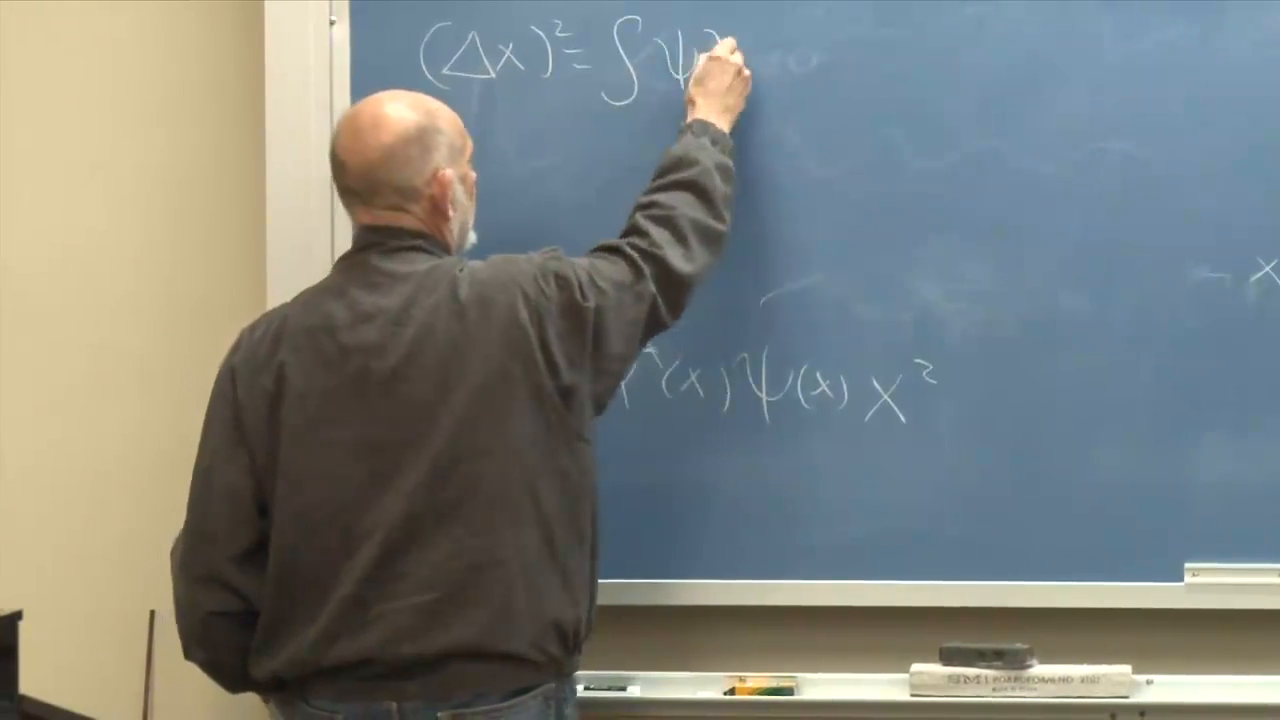
\includegraphics[width=0.88\textwidth]{lecture_10_figure_02.png}
\caption{Les fonctions d’onde en position et en impulsion sont les projections d’un même état sur deux bases continues différentes.}
\lectureframe{00:09:05}
\end{figure}

Dans deux dimensions spatiales, \(X\) et \(Y\) commutent ; une base propre commune peut donc être indexée par les deux coordonnées, et la fonction d’onde s’écrit \(\psi(x,y)\). Cette commutation ne découle pas des seuls axiomes abstraits : elle fait partie de la description quantique de l’espace ordinaire qui a été confirmée par l’expérience. Pour \(N\) particules dans trois dimensions,
\begin{equation}
\psi(\mathbf{x}_1,\ldots,\mathbf{x}_N)
\end{equation}
est une fonction sur l’espace des configurations, et non une fonction d’onde tridimensionnelle distincte attachée indépendamment à chaque particule. Un système macroscopique peut donc nécessiter un nombre énorme de coordonnées.

\begin{classroomqa}
\audiencequestion{La commutation de coordonnées spatiales différentes découle-t-elle automatiquement de la mécanique quantique ?}
\lecturerresponse{Non. Le cadre abstrait admet de nombreuses algèbres d’observables. La commutation de composantes cartésiennes distinctes de la position est un fait structurel empirique de la mécanique quantique des particules dans l’espace ordinaire.}
\end{classroomqa}

On peut effectuer une transformée de Fourier sur toutes les coordonnées pour obtenir une fonction d’onde de toutes les impulsions, ou ne transformer que certaines variables. Les représentations mixtes sont légitimes, car une représentation est un choix de base, et non un changement de l’état physique.

\section{Ce que mesure l’incertitude}

La forme la plus élémentaire du principe d’incertitude découle immédiatement de la paire de Fourier. Un état d’impulsion déterminée est une onde plane de module constant, sans localisation en position. Un état fortement localisé en position nécessite de nombreuses composantes d’impulsion. Plus généralement, resserrer la distribution d’un membre d’une paire de Fourier élargit celle de l’autre.

\begin{figure}[htbp]
\centering
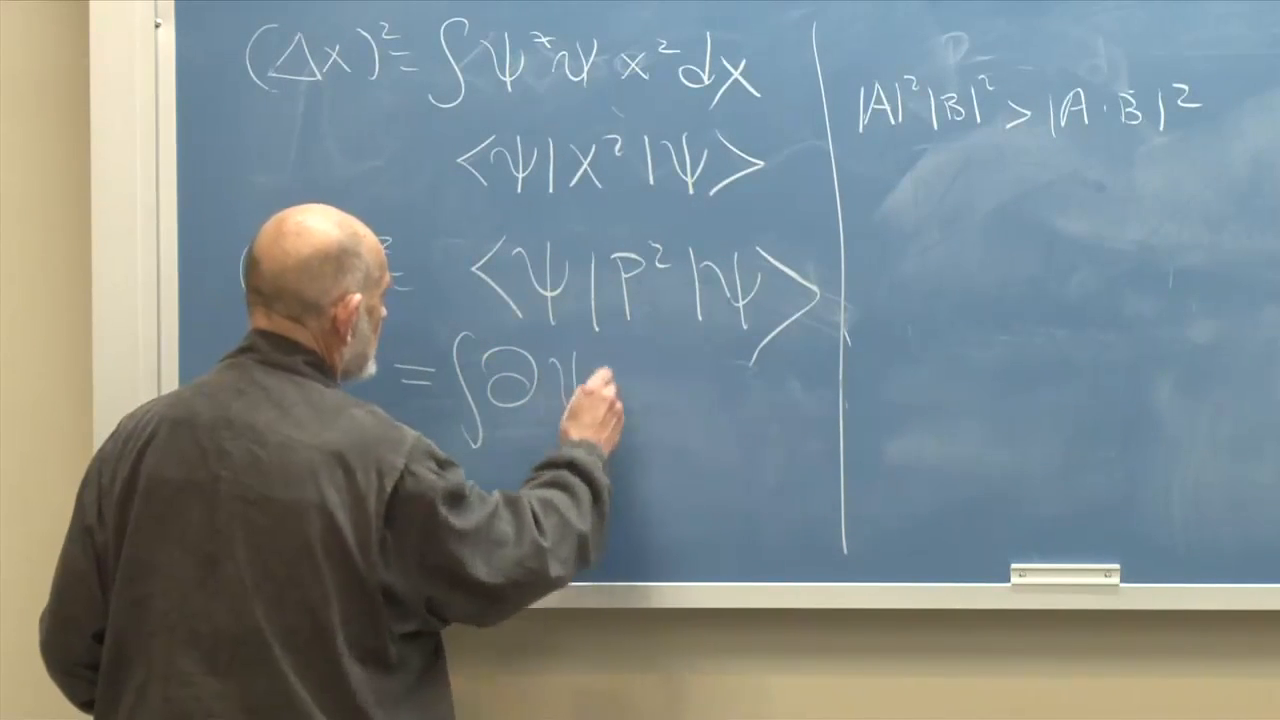
\includegraphics[width=0.88\textwidth]{lecture_10_figure_03.png}
\caption{Un profil de position localisé nécessite une large superposition d’ondes planes dans la représentation d’impulsion réciproque.}
\lectureframe{00:14:45}
\end{figure}

Pour quantifier cette affirmation, considérons une observable générale \(Q\). Sa valeur moyenne dans un état normalisé est
\begin{equation}
\expect{Q}=\bra{\psi}Q\ket{\psi}.
\end{equation}
La variance est
\begin{equation}
(\Delta Q)^2
=
\expect{\bigl(Q-\expect{Q}\bigr)^2}
=
\expect{Q^2}-\expect{Q}^2.
\label{eq:l10-general-variance}
\end{equation}
L’incertitude \(\Delta Q\) est la racine carrée positive de cette variance.

Pour la position, on peut d’abord décaler l’origine de sorte que \(\expect{X}=0\). Alors
\begin{equation}
(\Delta x)^2
=
\expect{X^2}
=
\int_{-\infty}^{\infty}
dx\,|\psi(x)|^2x^2.
\label{eq:l10-position-variance}
\end{equation}
Les contributions positives et négatives s’annulent dans \(\expect{X}\), mais s’additionnent dans \(\expect{X^2}\). Une distribution de probabilité plus étalée a donc une variance plus grande.

\begin{figure}[htbp]
\centering
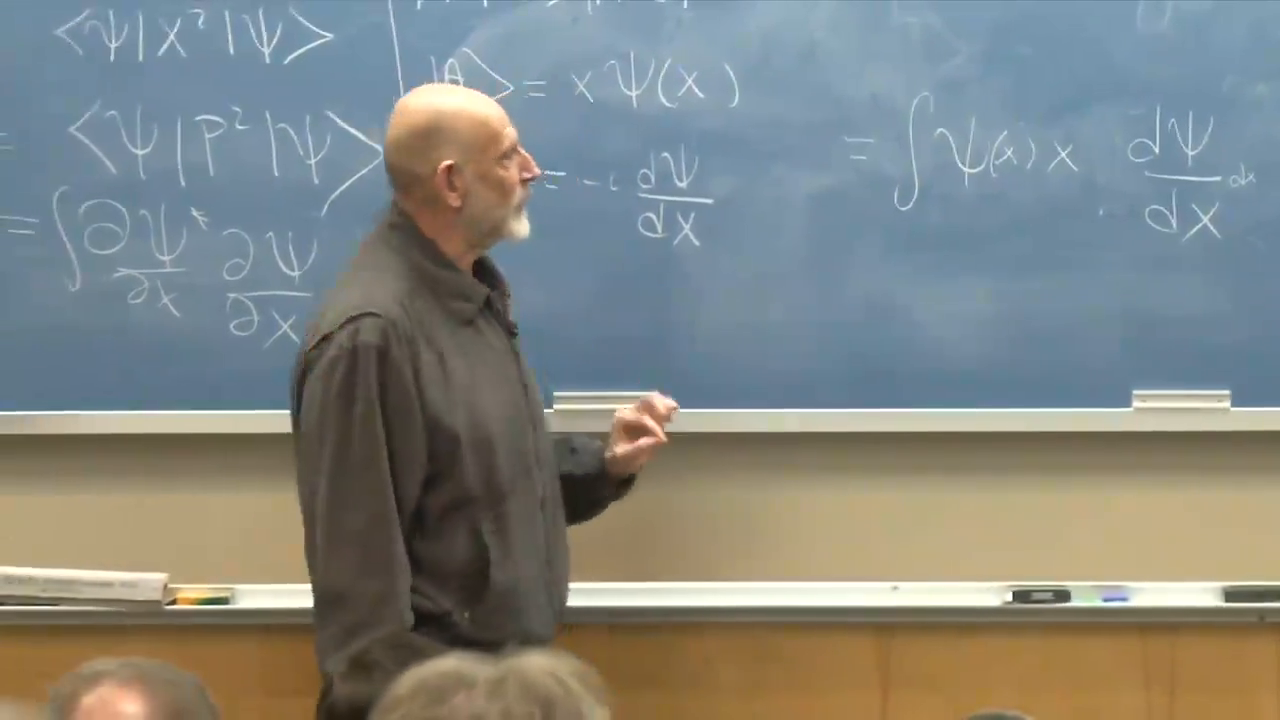
\includegraphics[width=0.88\textwidth]{lecture_10_figure_04.png}
\caption{Lorsque la moyenne est ramenée à zéro, la variance de position est l’intégrale de \(x^2\) pondérée par la probabilité.}
\lectureframe{00:20:50}
\end{figure}

La distinction entre \(\expect{X^2}\) et \(\expect{X}^2\) est essentielle. Une distribution symétrique par rapport à zéro vérifie \(\expect{X}=0\), mais, sauf si elle est concentrée à l’origine, elle vérifie tout de même \(\expect{X^2}>0\).

On peut définir directement la variance de l’impulsion dans l’espace des impulsions :
\begin{equation}
(\Delta p)^2
=
\int_{-\infty}^{\infty}
dp\,|\widetilde{\psi}(p)|^2
\bigl(p-\expect{P}\bigr)^2.
\end{equation}
Pour la démonstration, il est plus utile de travailler dans l’espace des positions. Ramenons la quantité moyenne d’impulsion à zéro et utilisons
\begin{equation}
P=-i\hbar\frac{d}{dx},
\qquad
P^2=-\hbar^2\frac{d^2}{dx^2}.
\end{equation}
On obtient alors
\begin{equation}
(\Delta p)^2
=
\expect{P^2}
=
-\hbar^2
\int_{-\infty}^{\infty}
dx\,\psi^*(x)\frac{d^2\psi}{dx^2}.
\label{eq:l10-momentum-variance-second}
\end{equation}

\begin{classroomqa}
\audiencequestion{Comment une variance peut-elle être positive si sa formule en représentation de position commence par un signe moins ?}
\lecturerresponse{L’intégrale qui multiplie ce signe est non positive. Une intégration par parties transfère une dérivée sur \(\psi^*\), introduit un second signe moins et transforme le résultat en l’intégrale d’un carré de module.}
\end{classroomqa}

Pour des fonctions d’onde qui décroissent assez rapidement à l’infini,
\begin{equation}
\int f\,g'\,dx
=
\left[fg\right]_{-\infty}^{\infty}
-
\int f'g\,dx,
\end{equation}
et le terme de bord s’annule. En appliquant cette relation une fois à l’équation~\eqref{eq:l10-momentum-variance-second}, on obtient
\begin{equation}
(\Delta p)^2
=
\hbar^2
\int_{-\infty}^{\infty}
dx\,
\frac{d\psi^*}{dx}
\frac{d\psi}{dx}
=
\hbar^2
\int_{-\infty}^{\infty}
dx\,
\left|\frac{d\psi}{dx}\right|^2
\geq 0.
\label{eq:l10-momentum-variance-positive}
\end{equation}

\begin{figure}[htbp]
\centering
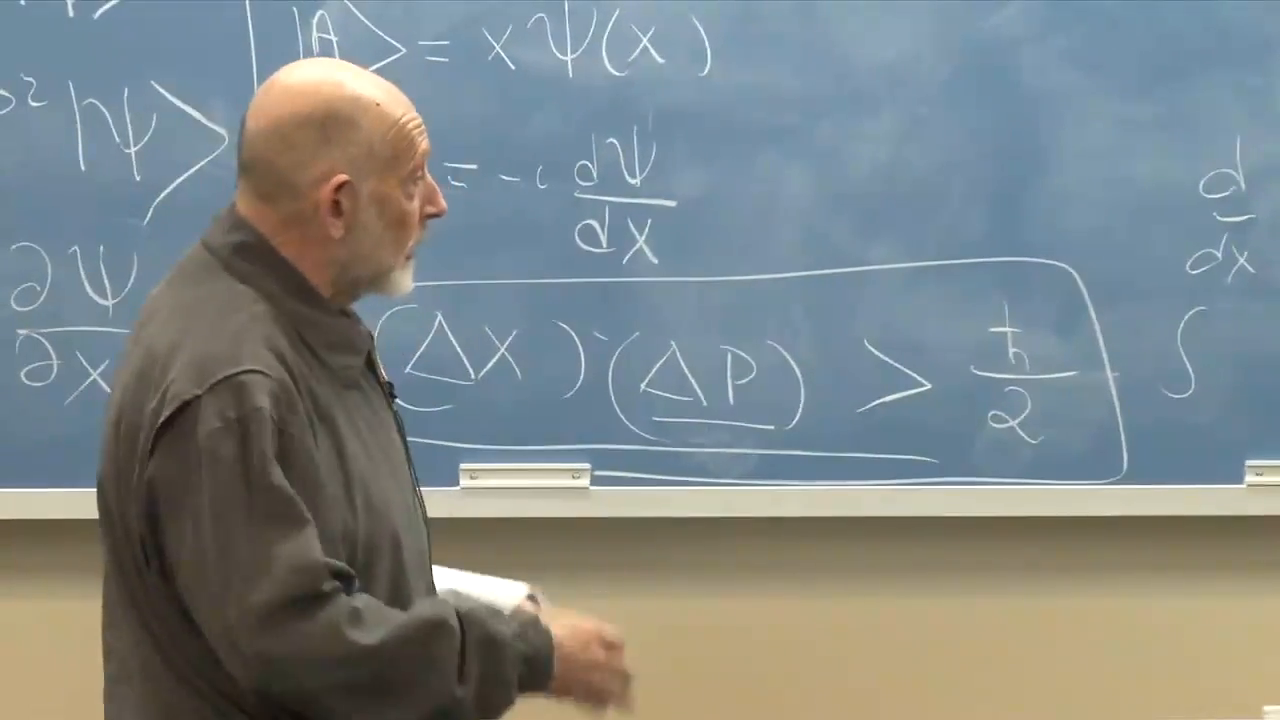
\includegraphics[width=0.88\textwidth]{lecture_10_figure_05.png}
\caption{L’intégration par parties transforme l’expression apparemment négative de \(\expect{P^2}\) en une norme manifestement positive.}
\lectureframe{00:27:35}
\end{figure}

\begin{classroomqa}
\audiencequestion{Peut-on ramener simultanément à zéro les valeurs moyennes de la position et de l’impulsion ?}
\lecturerresponse{Oui. La translation de l’argument de la fonction d’onde déplace \(\expect{X}\), tandis que sa multiplication par une phase d’onde plane déplace \(\expect{P}\). Ces opérations modifient les valeurs moyennes sans changer les variances correspondantes ; on peut donc utiliser dans la démonstration les deux variables centrées.}
\end{classroomqa}

\section{La borne d’incertitude}

L’outil mathématique nécessaire est l’inégalité de Cauchy--Schwarz. Le cours l’aborde à partir de la géométrie élémentaire des vecteurs : leur produit scalaire est égal au produit de leurs normes par le cosinus de l’angle qui les sépare ; son module ne peut donc dépasser le produit de leurs normes. En notation d’espace de Hilbert,
\begin{equation}
\braket{A}{A}\braket{B}{B}
\geq
\left|\braket{A}{B}\right|^2.
\label{eq:l10-cauchy-schwarz}
\end{equation}
Cette inégalité vaut dans les espaces vectoriels réels ou complexes, quelle que soit leur dimension.

\begin{figure}[htbp]
\centering
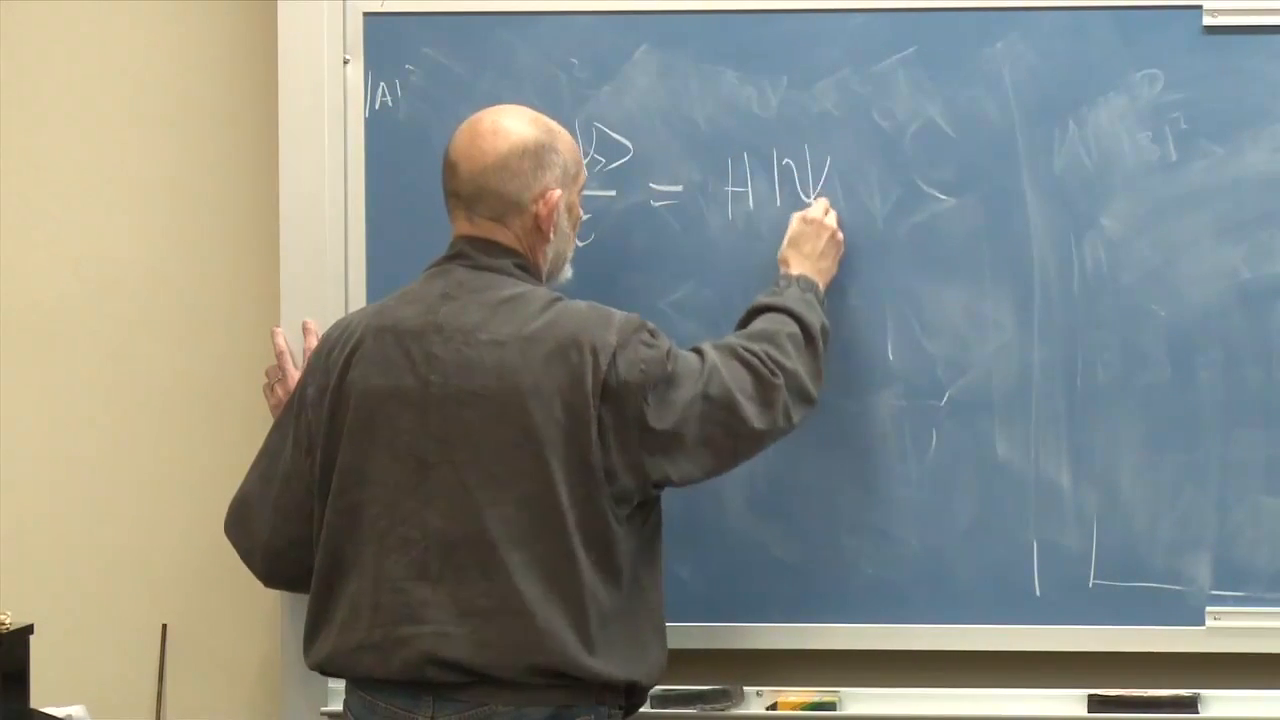
\includegraphics[width=0.88\textwidth]{lecture_10_figure_06.png}
\caption{L’inégalité géométrique sur les vecteurs est reformulée sous la forme de la borne de Cauchy--Schwarz dans l’espace de Hilbert, utilisée dans la démonstration.}
\lectureframe{00:35:35}
\end{figure}

\begin{classroomqa}
\audiencequestion{L’inégalité doit-elle être stricte, ou l’égalité est-elle possible ?}
\lecturerresponse{Il s’agit d’une relation supérieure ou égale. L’égalité se produit lorsque les deux vecteurs de l’espace de Hilbert sont linéairement dépendants. Cette condition d’égalité permettra ensuite d’identifier les paquets d’ondes d’incertitude minimale.}
\end{classroomqa}

Centrons les deux variables et suivons d’abord la démonstration simplifiée au tableau, qui suppose que \(\psi(x)\) est réelle. Définissons
\begin{equation}
\ket{A}=X\ket{\psi},
\qquad
\ket{B}=P\ket{\psi}.
\label{eq:l10-auxiliary-vectors}
\end{equation}
Leurs normes au carré sont précisément les variances :
\begin{equation}
\braket{A}{A}=(\Delta x)^2,
\qquad
\braket{B}{B}=(\Delta p)^2.
\end{equation}

\begin{figure}[htbp]
\centering
\includegraphics[width=0.88\textwidth]{lecture_10_figure_07.png}
\caption{Les vecteurs auxiliaires \(X\ket{\psi}\) et \(P\ket{\psi}\) expriment les deux variances sous forme de normes dans l’espace de Hilbert.}
\lectureframe{00:44:40}
\end{figure}

Le produit scalaire restant est
\begin{align}
\braket{A}{B}
&=
\int_{-\infty}^{\infty}
dx\,
x\psi(x)
\left(-i\hbar\frac{d\psi}{dx}\right).
\end{align}
Seule sa valeur absolue intervient. Puisque \(\psi\) est réelle,
\begin{equation}
\psi\frac{d\psi}{dx}
=
\frac{1}{2}\frac{d}{dx}\psi^2.
\end{equation}
Par conséquent,
\begin{align}
\left|\braket{A}{B}\right|
&=
\frac{\hbar}{2}
\left|
\int_{-\infty}^{\infty}
dx\,
x\frac{d}{dx}\psi^2
\right| \notag\\
&=
\frac{\hbar}{2}
\left|
-\int_{-\infty}^{\infty}
dx\,\psi^2
\right|
=
\frac{\hbar}{2},
\label{eq:l10-inner-product-half-hbar}
\end{align}
où l’intégration par parties élimine la dérivée de \(\psi^2\), \(d x/dx=1\), le terme de bord s’annule, et la normalisation donne la dernière égalité.

Insérons l’équation~\eqref{eq:l10-inner-product-half-hbar} dans l’inégalité de Cauchy--Schwarz :
\begin{equation}
(\Delta x)^2(\Delta p)^2
\geq
\frac{\hbar^2}{4}.
\end{equation}
En prenant la racine carrée positive, on obtient
\begin{equation}
\boxed{
\Delta x\,\Delta p
\geq
\frac{\hbar}{2}
}.
\label{eq:l10-uncertainty-principle}
\end{equation}

\begin{figure}[htbp]
\centering
\includegraphics[width=0.88\textwidth]{lecture_10_figure_08.png}
\caption{L’intégration par parties et la normalisation donnent la borne optimale d’incertitude entre position et impulsion.}
\lectureframe{00:50:55}
\end{figure}

La condition que \(\psi\) soit réelle était une commodité au tableau, et non une restriction du théorème. Pour un état complexe général, posons
\begin{equation}
\ket{A}=(X-\expect{X})\ket{\psi},
\qquad
\ket{B}=(P-\expect{P})\ket{\psi}.
\end{equation}
Le commutateur fixe la partie imaginaire de leur produit scalaire :
\begin{equation}
\operatorname{Im}\braket{A}{B}
=
\frac{1}{2i}\expect{[X,P]}
=
\frac{\hbar}{2}.
\end{equation}
Comme \(|\braket{A}{B}|\) est au moins égal au module de sa partie imaginaire, on obtient la même borne.

\begin{classroomqa}
\audiencequestion{Que devient exactement le terme de bord lors des intégrations par parties successives ?}
\lecturerresponse{Pour les paquets normalisables considérés ici, les produits qui apparaissent en \(+\infty\) et \(-\infty\) s’annulent. Sur un intervalle périodique fini, les termes aux extrémités se compensent. Le domaine des opérateurs doit être choisi de façon que ces propriétés soient vérifiées ; sinon, la manipulation formelle n’est pas justifiée.}
\end{classroomqa}

\begin{classroomqa}
\audiencequestion{Le signe d’égalité est-il physiquement réalisable, ou la borne inférieure n’est-elle qu’une estimation ?}
\lecturerresponse{Il est réalisable. L’égalité dans l’inégalité de Cauchy--Schwarz exige que les deux vecteurs auxiliaires soient proportionnels. La résolution de cette condition donne des paquets gaussiens, les états d’incertitude minimale étudiés ensuite.}
\end{classroomqa}

\section{Autres paires de variables conjuguées de Fourier}

La relation d’incertitude entre le temps et l’énergie ressemble à celle qui relie la position et l’impulsion. Elle demande toutefois plus de précautions, car le temps est généralement ici un paramètre d’évolution, et non une observable représentée par un opérateur universel auto-adjoint. Développons un état sur les vecteurs propres de l’énergie :
\begin{equation}
\ket{\psi(t)}
=
\int dE\,
\phi(E)e^{-iEt/\hbar}\ket{E}.
\label{eq:l10-time-energy-fourier}
\end{equation}
Les amplitudes en énergie et la variation temporelle sont reliées par une transformée de Fourier. Une distribution d’énergie étroite évolue lentement et ne peut produire une impulsion temporelle très brève ; une distribution d’énergie large peut donner une enveloppe d’arrivée brève.

\begin{figure}[htbp]
\centering
\includegraphics[width=0.88\textwidth]{lecture_10_figure_09.png}
\caption{La dépendance temporelle est construite à partir d’états propres de l’énergie munis des phases \(e^{-iEt/\hbar}\), qui fournissent la base de Fourier de la relation temps-énergie.}
\lectureframe{00:53:40}
\end{figure}

\begin{classroomqa}
\audiencequestion{La même démonstration s’applique-t-elle directement au temps et à l’énergie ?}
\lecturerresponse{L’intuition des largeurs réciproques s’applique, et un paquet d’ondes en propagation en donne un exemple utile : une fenêtre d’arrivée brève exige une large distribution d’énergie. L’énoncé en termes d’opérateurs est plus subtil, car le temps n’intervient pas dans cette formulation exactement comme \(X\).}
\end{classroomqa}

L’angle et le moment cinétique forment une autre paire de variables conjuguées pour le mouvement de rotation. Localement, leur relation de Fourier ressemble à celle entre la position et l’impulsion. À l’échelle globale, la périodicité de l’angle impose des précautions supplémentaires ; il s’agit donc ici d’une analogie, et non d’un théorème complet.

\begin{classroomqa}
\audiencequestion{Les paires position-impulsion, temps-énergie et angle-moment cinétique sont-elles des exemples isolés ?}
\lecturerresponse{Non. Les variables canoniquement conjuguées se présentent régulièrement comme des paires de Fourier. Les détails liés aux domaines et à la périodicité diffèrent, mais la localisation réciproque constitue leur structure commune.}
\end{classroomqa}

\section{L’équation de Schr\"odinger en représentation de position}

Revenons maintenant à la dynamique. La loi abstraite est
\begin{equation}
i\hbar\frac{d}{dt}\ket{\psi(t)}
=
H\ket{\psi(t)}.
\label{eq:l10-abstract-schrodinger}
\end{equation}
Pour une particule de masse \(m\) dans un potentiel \(V(X)\), prenons
\begin{equation}
H=\frac{P^2}{2m}+V(X).
\label{eq:l10-particle-hamiltonian}
\end{equation}
On reprend ainsi la forme classique, somme des termes cinétique et potentiel, puis on vérifie si son évolution quantique reproduit le mouvement classique dans le régime approprié.

\begin{figure}[htbp]
\centering
\includegraphics[width=0.88\textwidth]{lecture_10_figure_10.png}
\caption{L’Hamiltonien agit sur le vecteur d’état abstrait dans l’équation de Schr\"odinger dépendant du temps.}
\lectureframe{00:59:05}
\end{figure}

Dans la représentation de position, \(P^2\) devient une dérivée seconde. Une fonction de \(X\) agit par multiplication :
\begin{equation}
\bigl(V(X)\psi\bigr)(x)=V(x)\psi(x).
\end{equation}
Par conséquent,
\begin{equation}
i\hbar\frac{\partial\psi(x,t)}{\partial t}
=
\left[
-\frac{\hbar^2}{2m}\frac{\partial^2}{\partial x^2}
+V(x)
\right]\psi(x,t).
\label{eq:l10-position-schrodinger}
\end{equation}

\begin{figure}[htbp]
\centering
\includegraphics[width=0.88\textwidth]{lecture_10_figure_11.png}
\caption{L’Hamiltonien de la particule devient la dérivée seconde cinétique, à laquelle s’ajoute la multiplication par \(V(x)\).}
\lectureframe{01:03:05}
\end{figure}

\begin{classroomqa}
\audiencequestion{En quel sens la fonction ordinaire \(V(x)\) est-elle un opérateur ?}
\lecturerresponse{Une fois une base de position choisie, \(X\) agit par multiplication par \(x\). Toute fonction suffisamment régulière \(V(X)\) agit donc par multiplication par le nombre correspondant \(V(x)\) en chaque point. Son utilité se vérifie à partir de la dynamique qui suit.}
\end{classroomqa}

Pour calculer les valeurs moyennes, résolvons l’équation~\eqref{eq:l10-position-schrodinger} en fonction des deux dérivées temporelles :
\begin{align}
\dot{\psi}
&=
\frac{i\hbar}{2m}\psi''
-\frac{i}{\hbar}V\psi,
\label{eq:l10-psi-dot}\\
\dot{\psi}^{\,*}
&=
-\frac{i\hbar}{2m}\psi^{*\,\prime\prime}
+\frac{i}{\hbar}V\psi^*.
\label{eq:l10-psi-star-dot}
\end{align}
La deuxième ligne n’est que le conjugué complexe de la première, mais écrire les deux rend les simplifications visibles.

\section{Mouvement du centre du paquet}

Le centre de la distribution de position est
\begin{equation}
\expect{X}
=
\int_{-\infty}^{\infty}
dx\,\psi^*(x,t)\,x\,\psi(x,t).
\end{equation}
Dérivons cette expression :
\begin{equation}
\frac{d}{dt}\expect{X}
=
\int dx\,
\left(
\dot{\psi}^{\,*}x\psi
+
\psi^*x\dot{\psi}
\right).
\label{eq:l10-x-expectation-derivative}
\end{equation}
Les deux termes sont conjugués complexes. En substituant les équations~\eqref{eq:l10-psi-dot} et \eqref{eq:l10-psi-star-dot}, les termes de potentiel s’annulent parce que \(V(x)\) est réelle. Une intégration par parties des termes cinétiques donne
\begin{align}
\frac{d}{dt}\expect{X}
&=
\frac{1}{m}
\int dx\,
\psi^*
\left(-i\hbar\frac{\partial}{\partial x}\right)
\psi \notag\\
&=
\frac{\expect{P}}{m}.
\label{eq:l10-ehrenfest-x}
\end{align}

\begin{figure}[htbp]
\centering
\includegraphics[width=0.88\textwidth]{lecture_10_figure_12.png}
\caption{La dérivée du centre du paquet se réduit à la valeur moyenne de l’impulsion divisée par la masse.}
\lectureframe{01:15:40}
\end{figure}

Cette relation est exacte. Aucun rapprochement de paquet étroit n’est intervenu dans le calcul.

\begin{classroomqa}
\audiencequestion{Où a-t-on supposé, dans cette démonstration, que le paquet d’ondes est une seule bosse étroite ?}
\lecturerresponse{Nulle part. L’identité \(d\expect{X}/dt=\expect{P}/m\) est valable pour tout état appartenant au domaine de cet Hamiltonien. La localisation n’intervient que lorsque l’on interprète \(\expect{X}\) comme la trajectoire d’une particule classique.}
\end{classroomqa}

L’autre moitié de la mécanique concerne l’impulsion :
\begin{equation}
\expect{P}
=
\int dx\,
\psi^*
\left(-i\hbar\frac{\partial}{\partial x}\right)
\psi.
\end{equation}
Dérivons chacun des deux facteurs qui dépendent du temps :
\begin{equation}
\frac{d}{dt}\expect{P}
=
-i\hbar
\int dx\,
\left(
\dot{\psi}^{\,*}\psi'
+
\psi^*\frac{\partial\dot{\psi}}{\partial x}
\right).
\label{eq:l10-p-expectation-start}
\end{equation}
Après avoir intégré un terme par parties, substituons les deux équations de Schr\"odinger. Les contributions cinétiques s’annulent. Les termes de potentiel se regroupent en
\begin{equation}
\int dx\,
V(x)
\left(
\psi\frac{\partial\psi^*}{\partial x}
+
\psi^*\frac{\partial\psi}{\partial x}
\right)
=
\int dx\,
V(x)\frac{\partial}{\partial x}|\psi|^2.
\end{equation}
Une dernière intégration par parties transfère la dérivée au potentiel :
\begin{align}
\frac{d}{dt}\expect{P}
&=
-\int dx\,|\psi(x,t)|^2\frac{dV}{dx} \notag\\
&=
-\expect{V'(X)}
\\
&=
\expect{F(X)},\\
F(x)&=-V'(x).
\label{eq:l10-ehrenfest-p}
\end{align}

\begin{figure}[htbp]
\centering
\includegraphics[width=0.88\textwidth]{lecture_10_figure_13.png}
\caption{Les termes de potentiel se regroupent en une dérivée totale, ce qui donne \(d\expect{P}/dt=-\expect{V'(X)}\).}
\lectureframe{01:30:45}
\end{figure}

Les équations~\eqref{eq:l10-ehrenfest-x} et \eqref{eq:l10-ehrenfest-p} constituent le théorème d’Ehrenfest pour cet Hamiltonien. Ce sont des identités quantiques exactes, mais des équations exactes pour les valeurs moyennes ne décrivent pas encore une orbite classique.

\section{Où intervient l’approximation classique}

La mécanique classique appliquée à un point situé au centre du paquet exigerait
\begin{equation}
\frac{d}{dt}\expect{P}
\approx
F\!\left(\expect{X}\right).
\label{eq:l10-classical-center-force}
\end{equation}
La mécanique quantique donne plutôt
\begin{equation}
\frac{d}{dt}\expect{P}
=
\expect{F(X)}.
\end{equation}
En général,
\begin{equation}
\expect{F(X)}
\neq
F\!\left(\expect{X}\right).
\label{eq:l10-force-nonlinearity}
\end{equation}

\begin{classroomqa}
\audiencequestion{Si les deux équations d’Ehrenfest sont exactes, pourquoi ne démontrent-elles pas déjà que tout état quantique suit les lois de Newton ?}
\lecturerresponse{Pour obtenir la loi de Newton appliquée au centre du paquet, il faut évaluer la force en ce centre. L’équation quantique exacte contient la moyenne de la force sur toute la distribution de probabilité. Ces deux quantités coïncident pour un paquet étroit dans un champ de force qui varie lentement, mais pas pour un état quelconque ni pour une force non linéaire.}
\end{classroomqa}

Le contre-exemple du cours rend la distinction manifeste. Posons \(F(x)=x^2\) et choisissons un état normalisé constitué de deux bosses étroites égales, centrées près de \(+a\) et de \(-a\). Par symétrie,
\begin{equation}
\expect{X}=0,
\qquad
F\!\left(\expect{X}\right)=0,
\end{equation}
tandis que
\begin{equation}
\expect{F(X)}
=
\expect{X^2}
\approx
a^2>0.
\end{equation}

\begin{figure}[htbp]
\centering
\includegraphics[width=0.88\textwidth]{lecture_10_figure_14.png}
\caption{Pour un paquet symétrique à deux bosses et \(F(x)=x^2\), la force en la moyenne s’annule, tandis que la force moyenne ne s’annule pas.}
\lectureframe{01:33:35}
\end{figure}

Pour un paquet unique et étroit centré en \(\bar{x}=\expect{X}\), développons la force :
\begin{equation}
F(X)
=
F(\bar{x})
+
F'(\bar{x})(X-\bar{x})
+
\frac{1}{2}F''(\bar{x})(X-\bar{x})^2
+\cdots.
\end{equation}
La valeur moyenne annule le terme linéaire :
\begin{equation}
\expect{F(X)}
=
F(\bar{x})
+
\frac{1}{2}F''(\bar{x})(\Delta x)^2
+\cdots.
\end{equation}
L’approximation classique est fiable si le paquet reste étroit par rapport à l’échelle de longueur sur laquelle la force varie de manière appréciable.

Des structures prononcées peuvent scinder un paquet et le diffuser. Un potentiel étendu et régulier tend à guider un paquet suffisamment localisé sans détruire sa forme en bosse unique ; un obstacle ponctuel, un cœur atomique ou une structure à l’échelle de la longueur d’onde peut produire des composantes réfléchies et diffractées.

\begin{figure}[htbp]
\centering
\includegraphics[width=0.88\textwidth]{lecture_10_figure_15.png}
\caption{Une structure du potentiel à une échelle inférieure à la largeur du paquet ou comparable à la longueur d’onde pertinente peut décomposer un paquet cohérent en composantes diffusées.}
\lectureframe{01:37:25}
\end{figure}

\begin{classroomqa}
\audiencequestion{Qu’est-ce qui rend un potentiel défavorable à un paquet classique ?}
\lecturerresponse{La question est une question d’échelle, et non de caractère. Des structures beaucoup plus fines que le paquet ou comparables à sa longueur d’onde résolvent la nature ondulatoire et produisent de la diffusion. Si le potentiel varie lentement à l’échelle du paquet, la force est presque constante sur son support et le centre suit l’équation classique.}
\end{classroomqa}

La masse compte également. Pour un paquet presque d’incertitude minimale,
\begin{equation}
\Delta x\,\Delta v
\sim
\frac{\hbar}{2m}.
\end{equation}
Une masse élevée permet à la fois une faible largeur spatiale et une dispersion modérée des vitesses. Les objets lourds peuvent donc rester fortement localisés tout en traversant des potentiels macroscopiques. Il s’agit d’un argument d’échelle, et non de l’affirmation que la masse suffit à déterminer si le mouvement est classique.

\begin{classroomqa}
\audiencequestion{Un électron peut-il parfois être assez massif, en ce sens, pour se comporter approximativement de façon classique ?}
\lecturerresponse{Oui, si le champ extérieur varie régulièrement à l’échelle du paquet d’ondes de l’électron. Entre de larges plaques de condensateur, par exemple, un paquet cohérent peut suivre l’accélération classique pendant un temps appréciable. À proximité de la structure coulombienne prononcée d’un noyau, le même électron présente une diffusion marquée.}
\end{classroomqa}

L’expérience de diffusion de Rutherford de 1911 apporte une leçon complémentaire. Les particules alpha qui rencontraient la distribution de charge compacte d’un noyau d’or étaient déviées sous de grands angles, révélant que la charge positive était concentrée dans une région très petite. Rutherford décrivait un faisceau de particules ; la mécanique quantique décrit l’amplitude incidente et ses composantes diffusées. Les expériences modernes de diffusion d’électrons et de photons présentent la même sensibilité aux échelles.

\begin{classroomqa}
\audiencequestion{Ce comportement ondulatoire lié à l’échelle est-il propre aux particules matérielles ?}
\lecturerresponse{Non. Les ondes électromagnétiques suivent les lois de l’optique géométrique lorsque l’indice de réfraction varie lentement sur une longueur d’onde. Un réseau de diffraction dont l’espacement est comparable à la longueur d’onde disperse l’onde dans des directions distinctes. Les électrons, les particules alpha, les photons et les autres excitations quantiques partagent cette relation entre longueur d’onde et structure.}
\end{classroomqa}

La limite classique n’est donc pas une loi distincte ajoutée à la mécanique quantique. Les équations exactes portant sur les valeurs moyennes contiennent déjà les relations classiques. Les trajectoires classiques émergent lorsque l’état reste localisé et que l’Hamiltonien varie assez régulièrement pour que la moyenne de la force soit pratiquement égale à sa valeur au centre du paquet.
